
% Chapter 3

\chapter{État de l'art} % 3rd chapter title

\label{Chapter3} % For referencing the chapter elsewhere, use \ref{Chapter3} 


%----------------------------------------------------------------------------------------

\section{Position du problème}
\label{sec:position}

Nous commençons par présenter une modélisation mathématique d'une plaque de glace (appelé floe) sur la mer. Six variables (locales) sont nécessaires pour décrire le floe occupant la région fermée de l'espace $\Omega$ (voir \cref{fig:floe}) : 
\begin{itemize}
    \item Un ouvert connexe $\omega \in \Rdeux$ décrivant la section longitudinale du floe ;
    \item Deux fonctions $\hplus, \hmoins \in \mathcal{F}(\omega, \Run)$ décrivant l'épaisseur du floe, telle que $\forall x \in \omega, \hmoins(x) \leq \hplus(x)$ ;
    \item Le centre de masse du floe $G(w)$ ;
    \item Deux vecteurs $\eun$ et $\edeux$ formant une base sur $\omega$.
\end{itemize}

\begin{figure}[!h]
    \centering
    \begin{subfigure}[b]{0.45\textwidth}
        \centering
        % 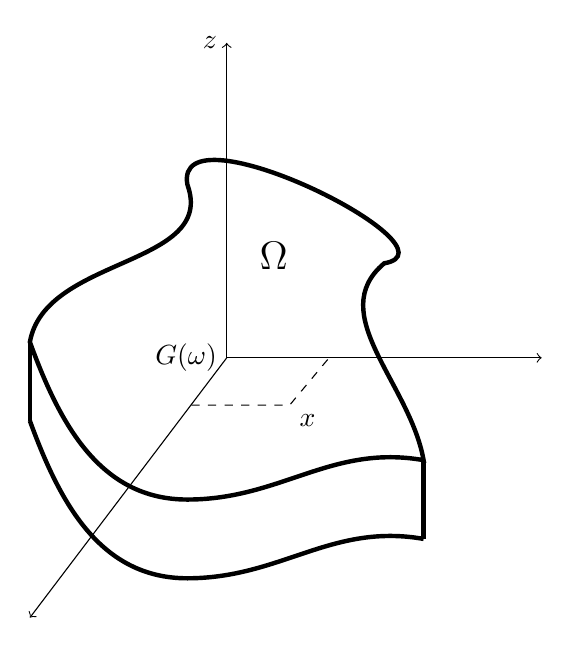
\begin{tikzpicture}
\node[coordinate] (v1) at (-3,3) {};
\node[coordinate] (v2) at (-5,1) {};
\node[coordinate] (v3) at (-3,-1) {};
\node[coordinate] (v4) at (0,-0.5) {};
\node[coordinate] (v5) at (-0.5,2) {};
%\draw  plot[smooth cycle, tension=.7] coordinates {(v5) (v1) (v2) (v3) (v4) (v5)};

\draw [ultra thick] (v1) to [out=290, in=80] (v2) to[out=290, in=180] (v3) to[out=0,in=170] (v4) to[out=100,in=220] (v5) to[out=10,in=100] (v1);

\node[coordinate] (v6) at (-5,0) {};
\node[coordinate] (v7) at (-3,-2) {};
\node[coordinate] (v8) at (0,-1.5) {};

\draw [ultra thick] (v2)--(v6); \draw [ultra thick] (v4)--(v8);
\draw [ultra thick]  (v6) to[out=290, in=180] (v7) to[out=0,in=170] (v8);

\node[coordinate] (v9) at (-2.5,0.8) {};
\node[coordinate] (v10) at (-5.0,-2.5) {};
\node[coordinate] (v11) at (1.5,0.8) {};
\node[coordinate] (v12) at (-2.5,4.8) {};

\draw [->] (v9)--(v10);
\draw [->] (v9)--(v11);
\draw [->] (v9)--(v12);


\node[left] (v9) at (-2.5,0.8) {$G(\omega)$};
\node[left] (v12) at (-2.5,4.8) {$z$};
\node[above left] (v13) at (-1.6,1.8) {\Large $\Omega$};

\node[coordinate] (v14) at (-1.2,0.8) {};
\node[coordinate] (v15) at (-1.7,0.2) {};
\node[coordinate] (v16) at (-2.95,0.2) {};
\draw[dashed] (v16)--(v15)--(v14);

\node[below right] (v15) at (-1.7,0.2) {$x$};

\end{tikzpicture}
        \includegraphics[width=.8\textwidth]{FloeVue1.tikz} 
        \caption{Vue d'un floe}
        \label{fig:floe1}
    \end{subfigure}
    % \hfill
    \begin{subfigure}[b]{0.45\textwidth}
        \centering
        % \usetikzlibrary{patterns}

\begin{tikzpicture}

\node[coordinate] (v0) at (0,0) {};
\node[coordinate] (v1) at (-5,0) {};
\node[coordinate] (v2) at (5,0) {};
\node[coordinate] (v3) at (0,-5) {};
\node[coordinate] (v4) at (0,5) {};

\draw [->] (v1)--(v2);
\draw [->] (v3)--(v4);

\node (v5) at (-4,2.5) {};
\node (v6) at (-1.5,3.5) {};
\node (v7) at (1,3.5) {};
\node (v8) at (3,2.5) {};
\node (v9) at (4,2.5) {};
\node (v10) at (-3.5,-2.5) {};
\node (v11) at (-2,-3.5) {};
\node (v12) at (-0.5,-3) {};
\node (v13) at (0.5,-3) {};
\node (v14) at (2,-3.5) {};
\node (v15) at (4.5,-3.5) {};

\draw[ultra thick]  plot[smooth, tension=.7] coordinates {(v5) (v6) (v7) (v8) (v9)};
\draw[ultra thick]  plot[smooth, tension=.7] coordinates {(v10) (v11) (v12) (v13) (v14) (v15)};

\draw [white, pattern=north east lines, xshift=0.5cm,yshift=4.5cm] plot coordinates {(v5) (v6) (v7) (v8) (v9) (v15) (v14) (v13) (v12) (v11) (v10) (v5)};

\node [above right] at (0,3.5) {\Large \bfseries $h_{+}(x)$};
\node [below right] at (0,-3.5) {\Large \bfseries $h_{-}(x)$};
\node [right] at (5,0) {\Large \bfseries $x$};
\node [left] at (0,5) {\Large \bfseries $z$};

\end{tikzpicture} 
        \includegraphics[width=.8\textwidth]{FloeVue2.tikz} 
        % \includegraphics[width=2cm]{Figures/FloeVue2.tex}
        \caption{Coupe transversale}
        \label{fig:floe2}
    \end{subfigure}
       \caption{Illustration de la géométrie d'un floe de glace $\Omega$.}
       \label{fig:floe}
\end{figure}

\noindent On confond le floe au volume qu'il occupe dans l'espace $\Omega$ :
\[
    \Omega = \{(x,z) \,|\, x \in \omega \in \Rdeux, \, z \in \,]\hmoins(x), \hplus(x)[ \, \} \,.
\] 
Les fonctions $\hmoins$ et $\hplus$ permettent de définir trois quantités (voir \cref{fig:h}) :
\begin{itemize}
    \item L'épaisseur moyenne du floe : $\bar{h} =  \sup_{x\in\omega}{\hplus(x)} - \inf_{x\in\omega}{\hmoins(x)}$ ;
    \item La plus forte épaisseur : $\bar{h}^* = \sup_{x\in\omega}{ \vert \hplus(x) - \hmoins(x) \vert}$ ;
    \item La plus faible épaisseur : $\underline{h}^* = \inf_{x\in\omega}{ \vert \hplus(x) - \hmoins(x) \vert}$. 
\end{itemize}

\begin{figure}[!h]
    \centering
    % \begin{tikzpicture}
	\begin{pgfonlayer}{nodelayer}
		\node [style=none] (0) at (0, 0) {};
		\node [style=none] (1) at (0, 5) {};
		\node [style=none] (2) at (0, -5) {};
		\node [style=none] (3) at (10, 0) {};
		\node [style=none] (4) at (-10, 0) {};
		\node [style=none] (5) at (-9.25, 2.5) {};
		\node [style=none] (6) at (-3.5, 1.5) {};
		\node [style=none] (7) at (3.25, 1.25) {};
		\node [style=none] (8) at (8.75, 4.75) {};
		\node [style=none] (9) at (-9, -6.75) {};
		\node [style=none] (10) at (-5, -4) {};
		\node [style=none] (11) at (2.5, -1.75) {};
		\node [style=none] (12) at (8.75, -1.25) {};
	\end{pgfonlayer}
	\begin{pgfonlayer}{edgelayer}
		\draw [->] (1.center) to (2.center);
		\draw [->] (4.center) to (3.center);
		\draw [bend right=15, looseness=0.75] (5.center) to (6.center);
		\draw [in=-165, out=0, looseness=1.25] (6.center) to (7.center);
		\draw [in=-135, out=15, looseness=1.25] (7.center) to (8.center);
		\draw [in=-165, out=45] (9.center) to (10.center);
		\draw [in=195, out=0, looseness=0.50] (10.center) to (11.center);
		\draw [in=180, out=15, looseness=0.75] (11.center) to (12.center);
	\end{pgfonlayer}
\end{tikzpicture}

    \includegraphics[width=.6\textwidth]{h.tikz}
    \caption{Différentes épaisseurs décrivant un floe de glace. Pour l'instant, afin d'obtenir un floe relativement plat (i.e $\bar{h}$ faible), $\hmoins$ sera pris identiquement nul, et $\hplus$ constant.}
    \label{fig:h}
\end{figure}

\noindent Les vecteurs $\eun$ et $\edeux$ sont liés à $\omega$, et pointent vers un point fixe du bord $\partial \omega$ du floe c-à-d :
\[
    \exists \sigma_i \in \partial \omega \, | \, e_i(\omega) = \frac{\sigma_i - G(\omega)}{\Vert \sigma_i - G(\omega) \Vert}, \text{ pour } i \in \{1,2\} \,,
\]
où $\Vert \cdot \Vert$ désigne la norme euclidienne de $\Rdeux$. Notons que $\sigma_1 \neq \sigma_2$, et $\eun \cdot \edeux = 0$ de façon à ce que la base orthonormée $(\eun, \edeux)$ soit directe.

Un floe $\Omega = (\omega, \eun, \edeux, G(\omega), \hmoins, \hplus)$ se déplace sur la mer\footnote{Pour l'instant, la mer est considérée comme un ouvert dans $\Rdeux$. Plus tard, nous prendrons en compte sont épaisseur lorsque nous la modéliserons par une sphère de $\Rtrois$.} $\mathcal{M} \in \Rdeux$. Au temps $t$ après une translation de vecteur $u(t)$ (et de matrice $\mathsf{T}_{u(t)}$), et une rotation de vecteur $\theta(t)$ (et de matrice $\bmat{R}_{\theta(t)}$), on obtient le floe $\Omega (t)$ défini par :
\[
    \Omega (t) = (\omega^\prime, \bvec e^1(\omega^\prime), \bvec e^2(\omega^\prime), G(\omega^\prime), \hmoins, \hplus) \,,
\]
avec
$$ 
\begin{cases}
    \omega^\prime = \bmat{T}_{u(t)} \bmat{R}_{\theta(t)} \omega \,, \\
    \bvec e_1(\omega^\prime) = \bmat{T}_{u(t)} \bmat{R}_{\theta(t)} \bvec e_1(\omega) \,, \\
    \bvec e_2(\omega^\prime) = \bmat{T}_{u(t)} \bmat{R}_{\theta(t)} \bvec e_2(\omega) \,, \\
    G(\omega^\prime) = \bmat{T}_{u(t)} \bmat{R}_{\theta(t)} G(\omega) \,.
\end{cases}
$$
C'est cette dernière notation mettant en exergue la dépendance avec le temps que nous utiliserons tout au long de ce rapport.

% \begin{figure}[!h]
%     \centering
%     % \begin{tikzpicture}
	\begin{pgfonlayer}{nodelayer}
		\node [style=none] (0) at (0, 0) {};
		\node [style=none] (1) at (0, 5) {};
		\node [style=none] (2) at (0, -5) {};
		\node [style=none] (3) at (10, 0) {};
		\node [style=none] (4) at (-10, 0) {};
		\node [style=none] (5) at (-9.25, 2.5) {};
		\node [style=none] (6) at (-3.5, 1.5) {};
		\node [style=none] (7) at (3.25, 1.25) {};
		\node [style=none] (8) at (8.75, 4.75) {};
		\node [style=none] (9) at (-9, -6.75) {};
		\node [style=none] (10) at (-5, -4) {};
		\node [style=none] (11) at (2.5, -1.75) {};
		\node [style=none] (12) at (8.75, -1.25) {};
	\end{pgfonlayer}
	\begin{pgfonlayer}{edgelayer}
		\draw [->] (1.center) to (2.center);
		\draw [->] (4.center) to (3.center);
		\draw [bend right=15, looseness=0.75] (5.center) to (6.center);
		\draw [in=-165, out=0, looseness=1.25] (6.center) to (7.center);
		\draw [in=-135, out=15, looseness=1.25] (7.center) to (8.center);
		\draw [in=-165, out=45] (9.center) to (10.center);
		\draw [in=195, out=0, looseness=0.50] (10.center) to (11.center);
		\draw [in=180, out=15, looseness=0.75] (11.center) to (12.center);
	\end{pgfonlayer}
\end{tikzpicture}

%     \includegraphics[width=.4\textwidth]{FloeMer.tikz}
%     \caption{Illustration du mouvement d'un floe de glace $F$ dans la mer, après une translation de vecteur $u(t)$ et une rotation d'angle $\theta(t)$, pour obtenir le floe $F_t$. On observe la transformation des propriétés du floe, en partucilier les vecteurs $e_1(\omega)$ et $e_2(\omega)$ qui restent liés au floe.}
% \end{figure}


Lors de leur mouvements sur la surface de la mer, les floes se fracturent sous l'effet des vents et des courants océaniques, des phénomènes thermodynamiques, etc. Nous nous intéresserons donc au phénomène de percussion en vue de l'initialisation des fractures dans les floes de glace. Afin de décrire le mouvement des floes de glace sur la mer, nous devons nous munir d'un repère absolu, que nous notons $\mathcal{R}_{abs} = (O, \bvec i, \bvec j, \bvec k)$. Le repère associé au floe $\Omega_i$ sera noté $\mathcal{R}_{\Omega_i} = (O, \bm \eun, \bvec \edeux, \bvec k)$. Dans ce repère absolu, le floe possède 3 degrés de libertés : l'abscisse et l'ordonné de son centre de gravité $G_i(\omega)$, et son orientation donnée par l'angle $\theta_i (t)$ (voir \cref{fig:FloeRepere}). 

\begin{figure}[!h]
    \centering
    % \begin{tikzpicture}
	\begin{pgfonlayer}{nodelayer}
		\node [style=none] (0) at (0, 0) {};
		\node [style=none] (1) at (0, 5) {};
		\node [style=none] (2) at (0, -5) {};
		\node [style=none] (3) at (10, 0) {};
		\node [style=none] (4) at (-10, 0) {};
		\node [style=none] (5) at (-9.25, 2.5) {};
		\node [style=none] (6) at (-3.5, 1.5) {};
		\node [style=none] (7) at (3.25, 1.25) {};
		\node [style=none] (8) at (8.75, 4.75) {};
		\node [style=none] (9) at (-9, -6.75) {};
		\node [style=none] (10) at (-5, -4) {};
		\node [style=none] (11) at (2.5, -1.75) {};
		\node [style=none] (12) at (8.75, -1.25) {};
	\end{pgfonlayer}
	\begin{pgfonlayer}{edgelayer}
		\draw [->] (1.center) to (2.center);
		\draw [->] (4.center) to (3.center);
		\draw [bend right=15, looseness=0.75] (5.center) to (6.center);
		\draw [in=-165, out=0, looseness=1.25] (6.center) to (7.center);
		\draw [in=-135, out=15, looseness=1.25] (7.center) to (8.center);
		\draw [in=-165, out=45] (9.center) to (10.center);
		\draw [in=195, out=0, looseness=0.50] (10.center) to (11.center);
		\draw [in=180, out=15, looseness=0.75] (11.center) to (12.center);
	\end{pgfonlayer}
\end{tikzpicture}

    \includegraphics[width=.5\textwidth]{FloeRepere.tikz}
    \caption{Positionnement d'un floe de glace $\Omega_i$ dans le repère absolu $\mathcal{R}_{abs}$.}
    \label{fig:FloeRepere}
\end{figure}


%----------------------------------------------------------------------------------------
\section{État de l'art}

Une fois le modèle défini, il nous faut établir les équations décrivant la dynamique du floe, et celle de son environnement. Les travaux de \cite{rabatel2015thesis} et \cite{balasoiu2020thesis} ont extensivement traité le problème de modélisation dynamique et de simulation d'un assemblage de floe de glace. Nous résumons ici les principales idées de leurs raisonnements, tout en présentant l'état de l'art dans ce domaine.

\subsection{Le modèle du floe}

\subsubsection{La cinétique du floe}

L'approche discrète décrite dans \parencite{rabatel2015thesis} utilise les mêmes notations que celles présentées à la \cref{sec:position}. Les obstacles\footnote{Nous faisons allusion aux obstacles au déplacement des floes. Il peut s'agir des iles, des stations offshore, etc.} sont des floes aux mêmes propriétés que les floes de glace, à la seule différence qu'ils ont une masse (volumique) infinie. Dans \parencite{rabatel2015thesis}, l'auteur travaille dans un repère orthonormé direct $\mathcal{R}_{abs} = (O, \bvec i, \bvec j, \bvec k)$ ; cependant, vu que la mer est considérée plane, le mouvement du floe peut être décrit dans le plan $\mathcal{P} = (O, \bvec i, \bvec j)$. Ensuite, \citeauthor{rabatel2015thesis} désigne la vitesse angulaire du floe $\Omega_i$ par 
$$
\bvec{\uptheta}_i(t) = \theta_i(t)\bvec{k} = (0,0,\theta_i(t))^T \,.
$$
Soit $P$ (de coordonné $x$) un point quelconque de $\P \subset \Rdeux$. Sa vitesse dans le repère $\R_{abs}$ est donnée est donnée par la formule de Varignon :
$$
\dot{P}(t) = \dot{G}_i(t) + \bm{\uptheta}_i(t) \wedge \bvec{G_iP} \,,
$$
où le symbole $\wedge$ représente le produit vectoriel dans $\Rtrois$. La masse (constante) du floe rigide indéformable est donnée par 
$$
M_i = \rho_i \int_{\Omega_i(t)} h_{i, +} (x) \diff x \,.
$$
Ensuite, l'auteur défini :
\begin{itemize}
    \item la somme des forces par unité de volume qui s'applique au centre de masse du floe $\Omega_i$ : $$\bvec{F}_i = \rho_i \int_{\Omega_i(t)} \bvec{F}(x) \diff x \,,$$
    \item le moment cinétique\footnote{Il s'agit d'un moment dû à l'accélération du floe ; alors que le moment dynamique est dû aux forces extérieures. Notons que ces deux vecteurs sont portés par $\bvec{k}$, et peuvent donc être remplacé par des scalaires correspondants.} en $G$ : $$L_i = \rho_i \intO{i} \bvec{GP} \wedge \dot{\bvec{P}}(t) \diff x \,,$$
    \item le moment dynamique en $G$ : $$\mathfrak{M}_i = \intO{i} \bvec{GP} \wedge \bvec{F}(x) \diff x \,.$$
\end{itemize}
Sous le formalisme de Newton-Euler, \citeauthor{rabatel2015thesis} montre que chaque floe $\Omega_i$ vérifie :
$$
% \begin{align}
    \begin{cases}
        M_i \frac{\diff \dot{\bvec{G}}_i(t)}{\diff t} &= \bvec{F}_i \\
        \mathcal{I}_i \frac{\diff \dot{\theta}_i(t)}{\diff t} &= \mathfrak{M}_i
    \end{cases} \,,
% \end{align}
$$
où $\mathcal{I}_i$ représente le moment d'inertie du floe $i$. Ce système se réécrit facilement sous la forme 
\begin{align}    
    \mathcal{M}_i \frac{\diff W_i(t)}{\diff t} = \mathcal{H}_i(t) \,,
\end{align}
avec 
$$
\mathcal{M}_i = 
\begin{pmatrix}
    M_i & 0 & 0 \\ 0 & M_i & 0 \\ 0 & 0 & \mathcal{I}_i
\end{pmatrix} \,, \quad
W_i(t) = 
\begin{pmatrix}
    \dot{\bvec{G}}(t) \\ \dot{\theta}_i(t)
\end{pmatrix} \,,
\text{ et } \quad \mathcal{H}_i(t) = 
\begin{pmatrix}
    \bvec{F}_i(t) \\ \mathfrak{M}_i(t)
\end{pmatrix} \,.
$$
Pour un système $S$ composé de $n$ floes, le problème précédent doit être satisfait pour tous les floes. \parencite[p.18]{rabatel2015thesis} montre que cela revient à résoudre l'équation
\begin{align} \label{eq:bilan1}
    \mathcal{M} \frac{\diff W(t)}{\diff t} = \mathcal{H}(t) \,,
\end{align}
avec 
$$
\mathcal{M} = (\mathcal{M}_i)_{1\leq i \leq n } \,, \quad
\mathcal{W}(t) = (\mathcal{W}_i(t))_{1\leq i \leq n } \,, \text{ et } \quad
\mathcal{M}(t) = (\mathcal{M}_i(t))_{1\leq i \leq n }  \,.
$$
L'énergie cinétique du floe $\Omega_i$ quant à elle sera donné par :
$$
E_i(t) = \frac{1}{2}M_i \dot{G}_i(t)^2 + \frac{1}{2}\mathfrak{I}_i \dot{\theta}_i(t)^2 \,. 
$$ 


\subsubsection{L'interaction entre les floes}


Le domaine de la mécanique du contact s'est grandement développé ces derniers siècles, avec plusieurs scientifiques qui ont tenté de décrire le phénomène de contact entre des corps rigides. Notons que le problème d'interaction entre les floes est un probleme de dynamique non-régulière (contraitement au probleme de éplacement des floes entre deux collisions qui lui, est un probleme de dynamqiue resguliere). Dans \parencite{rabatel2015thesis}, l'auteur considère deux lois de contact afin de décrire des phénomènes précis:
\begin{itemize}
    \item la condition unilatérale de Signorini: afin de décrire la condition de non-interpénétration;
    \item la loi de friction de Coulomb: afin de modéliser le comportement de friction pendant une collision.
\end{itemize}

Afin de traiter ces problemes de contact, deux approches principales ont été developpées par les scientifiques: l'approche non-régulière et l'approche de r;egularisation des lois de contact. 

Parmis les pioniers dans l'approche de régularisation pour la résolution de la condition unilatérale de Signorini, nous pourvons citer Hertz; Nevins et Whitney [NW72, Whi77], Moore [MW88b]; Ces méthodes se sont largement répandues dans les études liées à la robotique, à la réalité virtuelle ou encore dans les opérations assistées par ordinateur, pour simuler un grand nombre d’objets en contact en petites ou grandes déformations comme des habits, des cheveux ou encore des organes (voir [WW90, VCMT95, BW98, RGF+ 04]). Concernant la seconde, la loi de friction de Coulomb, la discontinuité entre les phases de glissement et non glissement a été traitée de différentes façons; en utilisant la notion de coefficeint de restitution, ou des modeles masse-ressorts. 
 
L'approche non-régulière a été développée en utilisant les concepts d'inclusion différentielles; ceci afin de traiter la condition de Signorini. Moreau [Mor85b], Aubin [AC84] et Monteiro Marques [MM85], ont montré des résultats d’existence et d’unicité de solutions du probleme sans friction. Puis, des résultats similaires ont été établis pour le contact unique avec friction (voir [Mor85a, MM88, Pan85, JP85, MM94]). Cependant, cette notion d'inclusion differentielle est difficile à manipuler; raison pour laquelle le problème du contact multiple avec friction reste encore très peu
traité.  Il a donc fallu attendre les années 80 avec l'essort des méthodes LCP pour doner un nouvau soufle à l'approche non régulière.Nous pouvons citer ici les travaux de Lötstedt qui des preuves d’existence et d’unicité pour le contact avec la friction de Coulomb (voir [Lot81, Lot82b, Lot82a]). On cite aussi Klarbring et Pang, pour leur apport sur le plan des méthodes de programmations. \parencite{rabatel2015thesis} a opté pour cette approche car elle facilite la construction des solutions à partir d’algorithmes tels que ceux de Lemke (voir [Lem78]). \citeauthor{rabatel2015thesis} s'insipire aussi des travaux de Baraff [Bar93], qui écrit les forces de contact dans les repères locaux aux points de contact. Ces repères sont définis par la normale et la tangente aux points de contact. La condition de complémentarité se résume comme ceci: "\textit{S’il y a contact alors la réaction est strictement positive et l’accélération relative nulle, et s’il n’y a pas contact l’accélération relative est strictement positive et la réaction nulle.
}". Cependant, les travaux de Baraff sur l'existence de solutions sont limités par l'approche accéleération-force qui est utilisée, et le coefficient de friction. En utilisant des formulations en vitesse et impulsion, les chercheurs ont réussi à démontrer l’existence de solutions pour toute configuration à contacts multiples avec n’importe quel coefficient de friction.


Pour traiter le problème de collision entre les floes, les glaciologues retiennent une multitude de  modèles principalement intégrés aux milieux continus. Par exemple, dans les articles de Solomon [Sol70], ceux de Hibler [HI79] et ceux de Bratchie [Bra84], la force résultante des interactions est due à une contrainte interne. On note aussi les modèles basés sur théorie des flux de particules. Dans
[SHL86, Hop85] par exemple, les collisions ne sont pas détectées précisément et les paramètres décrivant la collision sont déterminés par une méthode de Monte Carlo. L'introduction de ces déformations dans les modèles discrets de la banquise a été initié dans les années 90 par Hopkins [Hop96], et récement par Herman et Wilchinsky [Her11, WFH10]. Cependant, elles sont basées sur
la régularisation des lois de contact. Avant les travaux de \citeauthor{rabatel2015thesis}, il n'existait pas de modèle discret de banquise en utilisant une dynamique du contact non régulière.


Le modèle décrit par \parencite[p.5892]{rabatel2015dynamics} utilise deux conditions de complémentarité pour déterminer les vitesses des floes après le contact. La première est une condition de Signorini \parencite{signorini1933sopra} pour s'assurer de la non-interpénétration\footnote{Deux floes s'interpénètre si la "distance" entre ces deux floes est négative.} des floes. Pour décrire ces conditions, il faut au préalable écrire le problème de contact entre floes comme un problème implicite, où les inconnus sont les impulsions après le choc. Pour cette condition de complémentarité, \citeauthor{rabatel2015thesis} se base donc sur les travaux de Delassus (1917), Moreau (63), (Pfeiffer and Glocker, 1996). \citeauthor{rabatel2015thesis} se base ensuite sur les travaux de [Stewart and Trinkle, 1996] pour décrire une deuxième condition de complémentarité vérifiant la loi de fraction de Coulomb. Dans \parencite[p.5892]{rabatel2015dynamics}complémentarité. Le problème résultant a ensuite résolu en utilisant un algorithme de Lemke [Cottle et al., 1992, Alg. 6.3.1]. 

\textit{IMAGE D'UNE COLLISION EN Pj}

Soit $P_j$, ($j \in \{1,\ldots,n\}$) un point de contact entre les floes $\Omega_k$ et $\Omega_l$. Nous notons $\bvec{F}_{kj}(t)$ la force de contact du floe $\Omega_k$ au floe $\Omega_l$ appliquée en $P_j$. Par convention, une matrice de contact $\bmat{M_c}$ est définie telle que son coefficient $c_kj$ vaut :
\begin{itemize}
    \item $0\,\,\,\,\,\, $ si le point de contact $P_j$ n’est pas un point de contact du floe $\Omega_k$ ;
    \item $-1$ si le point de contact $P_j$ est un point de contact entre les floes $\Omega_k$ et $\Omega_l$ avec $k < l$ ;
    \item $1\,\,\,\,\,\, $ si le point de contact $P_j$ est un point de contact entre les floes $\Omega_k$ et $\Omega_l$ avec $k > l$.
\end{itemize}
En notant $E_k$ l’ensemble des points de contact du floe $\Omega_k$ au temps $t$, \parencite[p.26]{rabatel2015thesis} définit la résultante des forces de contact $\bvec{F}^c_k(t)$, au floe $\Omega_k$ comme :
$$
\bvec{F}^c_k(t) = \sum_{j \in E_k} c_{jk} \bvec{F}_{kj}(t) \,.
$$
En rajoutent ces forces aux forces extérieures lors du bilan des forces à l' \cref{eq:bilan1}, pour un floe $\Omega_k(t)$, on obtient :
\begin{align} \label{eq:bilan1}
    \mathcal{M} \frac{\diff W(t)}{\diff t} = \mathcal{H}(t) + \sum_{j \in E_k} \begin{pmatrix}
        \bvec{F}_{kj}(t) \\ \bvec{G^kP_j} \wedge \bvec{F}_{kj}(t) 
    \end{pmatrix} \,.
\end{align}


\subsubsection{Formulation en problème linéaire de complémentarité}

Il existe deux principales manières de formuler le problème du contact entre deux solides rigides. L'auteur de \parencite{rabatel2015thesis} opte pour le formalisme vitesse-impulsion, au détriment du formalisme accélération-force. En effet, L’approche en vitesse impulsion apporte l’avantage de pouvoir exprimer la force de friction de Coulomb directement par rapport à la vitesse. Il n’est pas nécessaire de connaître la nature du contact. Il nous faut donc définir les notions d'impulsion. Sur un intervalle de temps $\delta t^*$, s’il y a un contact entre les floes $\Omega_k$ et $\Omega_l$ au point $P_j$, nous dirons que le floe $\Omega_k$ a subi un choc provenant du floe $\Omega_l$ au point de contact $P_j$ caractérisé par l’impulsion :
$$
\bvec{\mathcal{I}}_{kj} = \int_{\delta t^*} c_{kj} \bvec{F}_{kj}(t) \diff t \,.
$$ 
\citeauthor{rabatel2015thesis} fait donc apparaître les impulsions dans les équations des moments \cref{eq:bilan1} pour le floe $\Omega_k$ sur l’intervalle temporel $\delta t^*$ :
$$
\mathcal{M}_k \int_{\dtstar} \dot{W}_k(t) \diff t = \int_{\dtstar} \mathcal{H}(t) \diff t + \sum_{j \in E_k} \begin{pmatrix}
    \bvec{\mathcal{I}}_{kj} \\ \bvec{G_kP_j} \wedge \bvec{\mathcal{I}}_{kj} 
\end{pmatrix} \,.
$$
En écrivant $\dtstar = [t^{-}, t^{+}]$, on peut donc introduire les inconnues $\beta$, $\lambda \in (\Rdeux)^m$ pour le problème de contact  
\begin{align}
    \mathcal{M} \left( W(t^{+}) - W(t^{-}) \right) = \int_{\dtstar} \mathcal{H}(t) \diff t + \bmat{B}\beta + \bmat{J}\lambda \,,
\end{align}
où $\bmat{B}$ et $\bmat{J}$ sont deux matrices de $(\Rtrois)^{n \times m}$telle que
\begin{align*}
    \bmat{B} = (d_{kj})_{\substack{1 \leq k \leq n \\ 1 \leq j \leq m}} \,, \quad d_{kj} = 
    \begin{cases}
        0 \in \Rtrois &\text{ si } P_j \text{ n'est pas un point de contact de } \Omega_k \\
        \begin{pmatrix}
            c_{kj} \bvec{T}_{j} \\ c_{kj} \bvec{P}_j\bvec{G}_k \wedge \bvec{T}_j 
        \end{pmatrix} &\text{ si } P_j \text{ est un point de contact de } \Omega_k
    \end{cases} \,, \\
    \bmat{J} = (s_{kj})_{\substack{1 \leq k \leq n \\ 1 \leq j \leq m}} \,, \quad s_{kj} = 
    \begin{cases}
        0 \in \Rtrois &\text{ si } P_j \text{ n'est pas un point de contact de } \Omega_k \\
        \begin{pmatrix}
            c_{kj} \bvec{N}_{j} \\ c_{kj} \bvec{P}_j\bvec{G}_k \wedge \bvec{N}_j 
        \end{pmatrix} &\text{ si } P_j \text{ est un point de contact de } \Omega_k
    \end{cases} \,.
\end{align*}
Les matrices $\bmat{B}$ et $\bmat{J}$ sont obtenues par décomposition des forces de contact dans le repère de contact $\mathcal{R}_{\Omega_j} = (P_j, \bvec{T}_j, \bvec{N}_j)$ (\textit{voir figure Plus Haut}).

Afin de modéliser la friction dans une collision qui respecte la loi de Coulomb, \parencite{rabatel2015thesis} se base sur les travaux de Stewart et Trinkle (96) qui définissent une condition de complémentarité reliant la composante tangentielle $\beta_j$ de l'impulsion appliquée au point $P_j$, la composante normale $\lambda_j$, la vitesse relative tangentielle du point $P_j$ et le coefficient de friction $\mu$. On introduit le vecteur $\tilde{\beta}$ contenant les composantes de l'impulsion tangentielle dans chacune des directions possible de glissement $\bvec{T}_j$ et $-\bvec{T}_j$. Il devient alors possible de formuler le problème de contact (sur tout le système $S$) sans interpénétration par le problème linéaire de complémentarité :
\begin{align} \label{eq:bilan3}
\begin{cases} \quad
    \begin{pmatrix}
        0 \\ \bvec{w} \\ \gamma \\ \sigma 
    \end{pmatrix} =  
    \begin{pmatrix}
        \mathcal{M} &  -\bmat{J} & -\bmat{D} & 0 \\
        \bmat{J}^T & 0 & 0 & 0 \\
        \bmat{D}^T & 0 & 0 & \bmat{H} \\
        0 & \mu & -\bmat{H}^T & 0
    \end{pmatrix} 
    \begin{pmatrix}
        W(t^+) \\ \lambda \\ \tilde{\beta} \\ \alpha
    \end{pmatrix} + 
    \begin{pmatrix}
        \int_{\delta t^*} \mathcal{H}(t) \diff t - \mathcal{M} W(t^{-}) \\ 0 \\ 0 \\ 0
    \end{pmatrix} \\ \quad
    \begin{pmatrix}
        \bvec{w} \\ \gamma \\ \sigma
    \end{pmatrix} \geq 0 \,, \quad
    \begin{pmatrix}
        \lambda \\ \tilde{\beta} \\ \alpha
    \end{pmatrix} \geq 0 \,, \quad
    \begin{pmatrix}
        \bvec{w} \\ \gamma \\ \sigma
    \end{pmatrix} \cdot
    \begin{pmatrix}
        \lambda \\ \tilde{\beta} \\ \alpha
    \end{pmatrix}  
     = 0 \,,
\end{cases}
\end{align}
avec
\begin{align*}
    &\bvec{w} = \bmat{J}^T W(t^+) \,, \quad
    \bmat{H}^T = (e_{ij})_{\substack{1 \leq i \leq m \\ 1 \leq j \leq 2m}} \,, \quad \tilde{\beta} = (\tilde{\beta}_j)_{1\leq j \leq m} \,, \quad \lambda = (\lambda_j)_{1 \leq j \leq m} \,, \\
    &\mu \text{ est la matrice diagonale de diagonale} (\mu_1,\dots, \mu_m) \,,\\
    &e_{ij} = \begin{cases}
        1 \text{   si } j = 2(i-1) + 1 \text{ ou } j=2(i-1) + 2 \\
        0 \text{   sinon} 
    \end{cases} \,,\\
    &D = (\bvec{B}_1 \vert - \bvec{B}_1 \vert \ldots \vert \bvec{B}_m \vert -\bvec{B}_m) \, \quad \text{ avec } \bvec{B}_j \text{ la colonne } j \text{ de la matrice } \bmat{B} \,.
\end{align*}
Le problème consiste alors à trouver les vitesses après contact $W(t^{+})$, à l’aide des composantes inconnues tangentielle et normale des impulsions dans les repères de contact $(\tilde{\beta}\, \gamma)$, elles-mêmes inconnues du système.

\subsubsection{Consistance énergétique}
D'après l'auteur de \parencite[p.42]{rabatel2015thesis}, traiter le problème de contact à partir de lois non régulières ne permet pas d’obtenir des solutions satisfaisant à la fois la non-interpénétration, la friction de Coulomb et une consistance énergétique. Le problème a donc été divisé en une phase de compression et une phase de décompression suivant la loi de Poisson, durant lesquelles un problème de complémentarité (\cref{eq:bilan3}) a été résolu. Durant la phase de décompression, \citeauthor{rabatel2015thesis} a donc opté pour la consistance énergétique et la non-interpénétration avec la solution :
$$
W^N = (1 + \varepsilon)W^{c} - \varepsilon W(t^{-}) \,,
$$
où $W^c$ représente les vitesses des floes après la phase de compression, et $\varepsilon$ le coefficient de restitution pour les contacts considérés inélastiques.

\subsubsection{Traitement des conditions aux bords}

\subsection{Le modèle de l'environnement}



